%% LaTeX2e class for student theses
%% sections/evaluation.tex
%% 
%% Karlsruhe Institute of Technology
%% Institute for Program Structures and Data Organization
%% Chair for Software Design and Quality (SDQ)
%%
%% Dr.-Ing. Erik Burger
%% burger@kit.edu
%%
%% Version 1.3.3, 2018-04-17

\chapter{Evaluation Via User Studies}
\label{ch:Evaluation}

\section{Experimental Settings}
\label{sec:Evaluation:ExperimentalSettings}
In this thesis, we compare three different visualization methods, namely the so-called “Heatmap”, “Bar Graph” and “Force-Direct-Graph”. The participants are assessed with respect to different conditions, to which they will be assigned randomly. Participants are not aware of the condition they are assigned to: 
\begin{itemize}
	\item \textbf{Condition A}: Participants can only use the Heatmap and \autoref{fig:mockup_hm} is its mock-up
	\begin{figure}[htb]
		\centering
		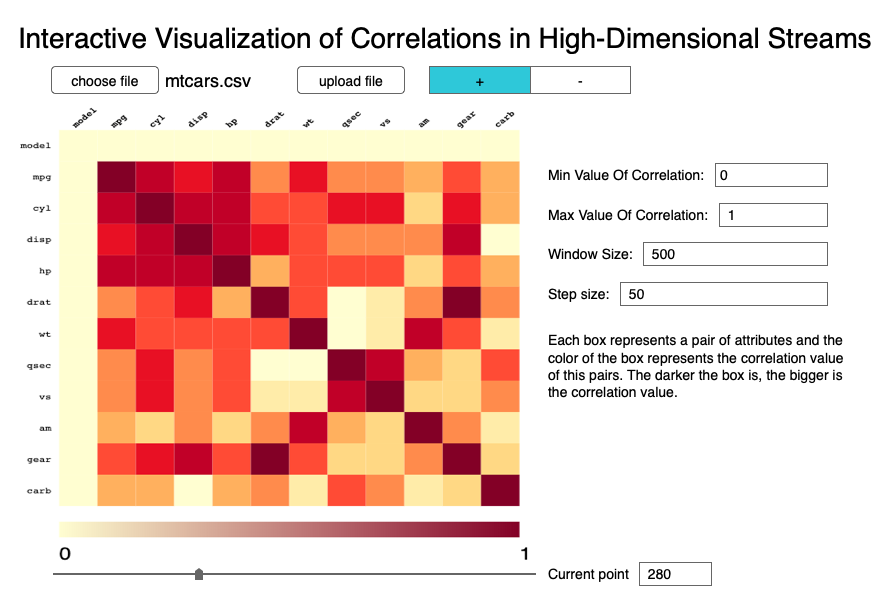
\includegraphics[width=15cm]{pictures/mockup_hm}
		\caption{Mock-up for Condition A}
		\label{fig:mockup_hm}
	\end{figure}

	\item \textbf{Condition B}: Participants can only use the Bar Graph and \autoref{fig:mockup_bg} is its mock-up
	\begin{figure}[htb]
		\centering
		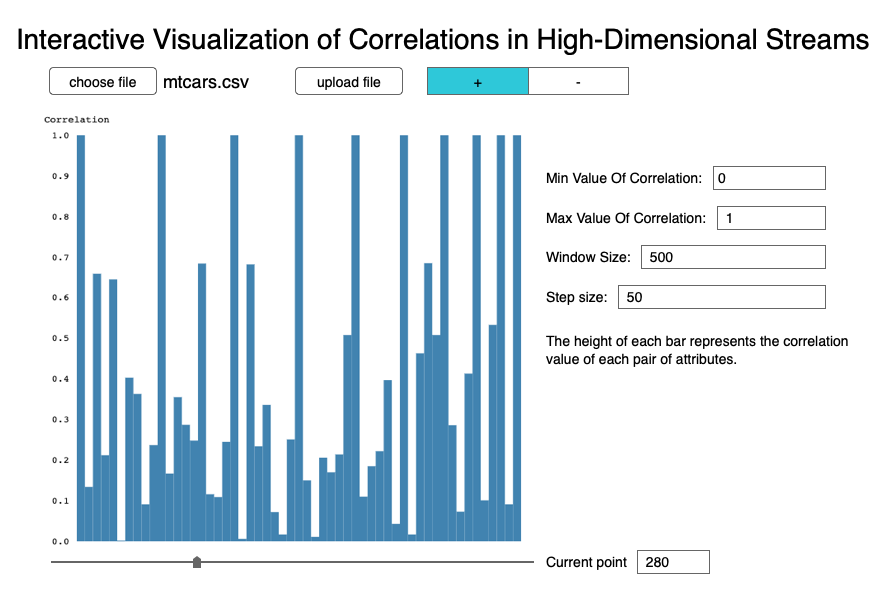
\includegraphics[width=15cm]{pictures/mockup_bg}
		\caption{Mock-up for Condition B}
		\label{fig:mockup_bg}
	\end{figure}
	
	\item \textbf{Condition C}: Participants can only use the Force-Directed-Graph and \autoref{fig:mockup_fdg} is its mock-up
	\begin{figure}[htb]
		\centering
		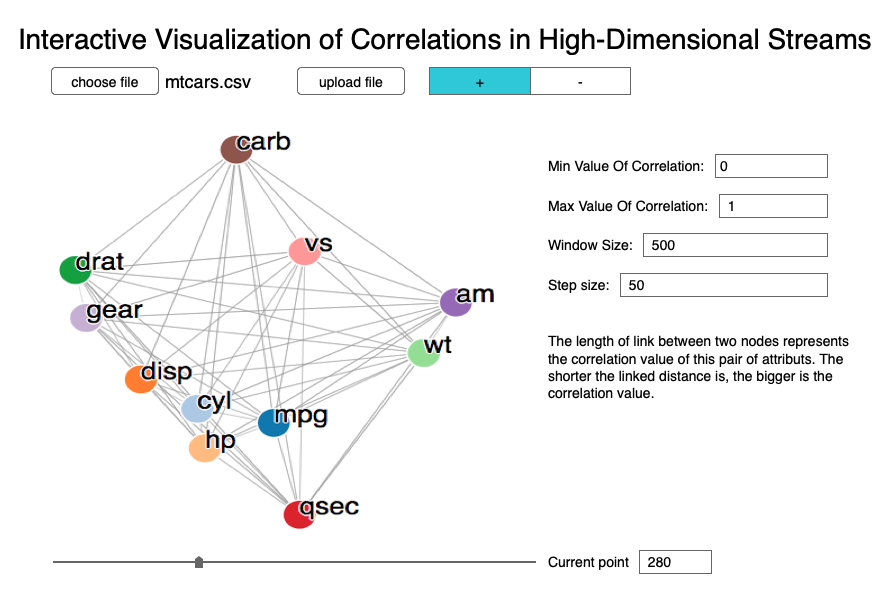
\includegraphics[width=15cm]{pictures/mockup_fdg}
		\caption{Mock-up for Condition C}
		\label{fig:mockup_fdg}
	\end{figure}
	
	\item \textbf{Condition D}: Participants can use any visualization method they want,which are mentioned in Condition A,B and C, and \autoref{fig:mockup} is its mock-up
		\begin{figure}[htb]
		\centering
		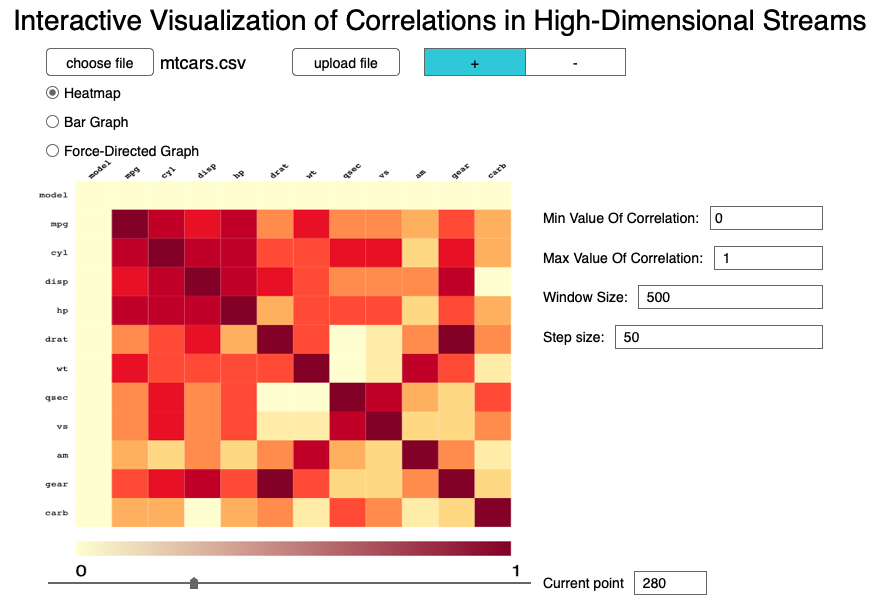
\includegraphics[width=15cm]{pictures/mockup_3}
		\caption{Mock-up for Condition D}
		\label{fig:mockup_3}
	\end{figure}
\end{itemize}

\subsection{Participants Profiles}
\label{sec:Evaluation:ExperimentalSettings:PP}
The participants we are looking for are adults who at least have the basic knowledge about browsing web page, typically 14 to 40 years old. We will sample a large share of our participants from the pool of students at KIT, so we may expect basic knowledge of computer science and data analysis.\\
Knowledge in data analysis and correlation analysis should not be required to use the prototype for the visualization of a data set. Still, we hypothesis that participants with prior exposure to data visualization will require less time to fulfill the tasks.\\

\subsection{Data Set}
\label{sec:Evaluation:ExperimentalSettings:DataSet}
The participant of user study are asked to use a data set taken at random from a pool of 3 data sets in total for completing the tasks. \textbf{Data Set 1 (DS1)} has 10 attributes within 2000 timestamps. \textbf{Data Set 2 (DS2)} has 20 attributes within 2000 timestamps. \textbf{Data Set 3 (DS3)} has 40 attributes within 2000 timestamps. These 3 data sets are actually the subsets of a real-world data set. For the evaluation, we make some modifications of this data set: reducing the number of attributes and selecting only 2000 instances of it. It is obvious that the difference between DS1, DS2 and DS3 are their level of difficulty according to their number of dimensions. In practice, this means that the same question will be harder to answer with DS3 than DS2 and DS1.\\

\subsection{Settings of interface}
The window size is set to 200 and the step size is set 50 for all three data sets, which cannot be changed by the participants.\\
During the user study, the participants are only able to change the minimum and maximum to filter the correlation values. Also, they can slide the sliding window or input "current point" to get the visualization graph of current timestamp.

\section{Questionnaire}
\label{sec:Evaluation:Questionnaire}
Before answering the questionnaire, all participants are asked to sign a Consent Form, shown in \autoref{cf}. The questionnaire is divided into 3 parts. In the first part of questionnaire \autoref{sec:Evaluation:Questionnaire}, the participants are asked to give some basic information. In the second part of questionnaire, the participants have to answer some questions using different visualization methods. \autoref{sec:Evaluation:Questionnaire:V} shows the question types and each question type will be asked three time in the user study. \autoref{sec:Evaluation:Questionnaire:F} is the last part of questionnaire, which introduces the feedback of using this interface. Participants under Condition A/B/C are asked to give feedback of the corresponding visualization methods they use, while participants under Condition D have to give feedback of each visualization method and the whole system.
\subsection{Basic Information}
\label{sec:Evaluation:Questionnaire:BI}
\begin{itemize}
	\item Field of study
	\item Number of semester
	\item Age:\\
	\begin{tabular}{| l | c | r |}
		\hline
		18-24 & 25-30 & More than 30 \\ \hline
	\end{tabular}
	\item Gender:\\
		\begin{tabular}{| l | c | r |}
		\hline
		M & F & Do not wish to answer \\ \hline
	\end{tabular}
	\item How familiar are you with the following concepts?
\begin{center}
	\begin{tabular}{ | l | l | l | l | l | l | l | l |}
		\hline
		                              & 1 (Unfamiliar) & 2 & 3 & 4 & 5 & 6 & 7 (Very Familiar) \\ \hline
		\textbf{Correlation analysis} &                &   &   &   &   &   &                   \\ \hline
		\textbf{Data analysis}        &                &   &   &   &   &   &                   \\ \hline
		\textbf{Data visualization}   &                &   &   &   &   &   &                   \\ \hline
	\end{tabular}
\end{center}
\end{itemize}

\subsection{Visualization}
\label{sec:Evaluation:Questionnaire:V}
\begin{itemize}
\item How many attributes are available in this data set?
\item How many pairs of attributes are available in this data set?
\item What is the correlation value between \textit{\textbf{\underline{Attribute A}}} and \textit{\textbf{\underline{Attribute B}}} at \textit{\textbf{\underline{Timestamp T}}}, or the probable range?
\item Which pair of attributes has the biggest correlation at \underline{\textbf{\textit{Timestamp T}}}?
\item Which pair of attributes has the smallest correlation at \underline{\textbf{\textit{Timestamp T}}}?
\item The following statement is true or false: “The correlation value between \underline{\textit{\textbf{Attribute A}}} and \underline{\textit{\textbf{Attribute B}}} remains the same at \underline{\textit{\textbf{Timestamp T1}}} and at \underline{\textit{\textbf{Timestamp T2}}}”?\\
	\begin{tabular}{| l | c |}
	\hline
	True & False \\ \hline
\end{tabular}
\item Which pair(s) of attributes has/have a correlation value that is not smaller than \underline{\textit{\textbf{X}}} at \underline{\textit{\textbf{Timestamp T}}}?
\item Which pair(s) of attributes has/have a correlation value that is not bigger than \underline{\textit{\textbf{X}}} at \underline{\textit{\textbf{Timestamp T}}}?
\end{itemize}

\subsection{Feedback}
\label{sec:Evaluation:Questionnaire:F}
\subsubsection{Participants Under Condition A/B/C}
Participants under Condition A, B and C are asked to give feedback based on following questions:
\begin{itemize}
	\item Please write down the visualization method you have used and rate for it.
	\begin{center}
		\begin{tabular}{ | l | l | l | l | l | l | l | l | }
			\hline
			                     & 1 (Strongly Disagree) & 2 & 3 & 4 & 5 & 6 & 7 (Strongly Agree) \\ \hline
			\textbf{Intuitive}   &                       &   &   &   &   &   &                    \\ \hline
			\textbf{Convenient}  &                       &   &   &   &   &   &                    \\ \hline
			\textbf{Interactive} &                       &   &   &   &   &   &                    \\ \hline
			\textbf{Useful}      &                       &   &   &   &   &   &                    \\ \hline
			\textbf{Complicated} &                       &   &   &   &   &   &                    \\ \hline
			\textbf{Efficient}   &                       &   &   &   &   &   &                    \\ \hline
			\textbf{Effective}   &                       &   &   &   &   &   &                    \\ \hline
		\end{tabular}
	\end{center}
\item In your opinion, what are the strengths of this visualization system?
\item In your opinion, what are the weaknesses of this visualization system?
\item Do you have any suggestions for improving this visualization system?
\end{itemize}

\subsubsection{Participants Under Condition D}
Participants under Condition D, who are able to use either of 3 visualization methods, are asked to give feedback to the whole system, which is also quite similar to the one for participants under Condition A, B or C. In addition, they need to give ratings for each visualization method.
\begin{itemize}
	\item As you are able to use all visualization methods during the research, which one of the method, in your opinion, is the most helpful method to fulfill the task?
	\item And which of the method did you use the most?
	\item Please rate for \textit{Heat map}:
		\begin{center}
		\begin{tabular}{ | l | l | l | l | l | l | l | l | }
			\hline
			& 1 (Strongly Disagree) & 2 & 3 & 4 & 5 & 6 & 7 (Strongly Agree) \\ \hline
			\textbf{Intuitive}   &                       &   &   &   &   &   &                    \\ \hline
			\textbf{Convenient}  &                       &   &   &   &   &   &                    \\ \hline
			\textbf{Interactive} &                       &   &   &   &   &   &                    \\ \hline
			\textbf{Useful}      &                       &   &   &   &   &   &                    \\ \hline
			\textbf{Complicated} &                       &   &   &   &   &   &                    \\ \hline
			\textbf{Efficient}   &                       &   &   &   &   &   &                    \\ \hline
			\textbf{Effective}   &                       &   &   &   &   &   &                    \\ \hline
		\end{tabular}
	\end{center}
		\item Please rate for \textit{Bar Graph}:
	\begin{center}
		\begin{tabular}{ | l | l | l | l | l | l | l | l | }
			\hline
			& 1 (Strongly Disagree) & 2 & 3 & 4 & 5 & 6 & 7 (Strongly Agree) \\ \hline
			\textbf{Intuitive}   &                       &   &   &   &   &   &                    \\ \hline
			\textbf{Convenient}  &                       &   &   &   &   &   &                    \\ \hline
			\textbf{Interactive} &                       &   &   &   &   &   &                    \\ \hline
			\textbf{Useful}      &                       &   &   &   &   &   &                    \\ \hline
			\textbf{Complicated} &                       &   &   &   &   &   &                    \\ \hline
			\textbf{Efficient}   &                       &   &   &   &   &   &                    \\ \hline
			\textbf{Effective}   &                       &   &   &   &   &   &                    \\ \hline
		\end{tabular}
	\end{center}
		\item Please rate for \textit{Force-Directed Graph}:
	\begin{center}
		\begin{tabular}{ | l | l | l | l | l | l | l | l | }
			\hline
			& 1 (Strongly Disagree) & 2 & 3 & 4 & 5 & 6 & 7 (Strongly Agree) \\ \hline
			\textbf{Intuitive}   &                       &   &   &   &   &   &                    \\ \hline
			\textbf{Convenient}  &                       &   &   &   &   &   &                    \\ \hline
			\textbf{Interactive} &                       &   &   &   &   &   &                    \\ \hline
			\textbf{Useful}      &                       &   &   &   &   &   &                    \\ \hline
			\textbf{Complicated} &                       &   &   &   &   &   &                    \\ \hline
			\textbf{Efficient}   &                       &   &   &   &   &   &                    \\ \hline
			\textbf{Effective}   &                       &   &   &   &   &   &                    \\ \hline
		\end{tabular}
	\end{center}
		\item Please rate for \textit{whole system}:
	\begin{center}
		\begin{tabular}{ | l | l | l | l | l | l | l | l | }
			\hline
			& 1 (Strongly Disagree) & 2 & 3 & 4 & 5 & 6 & 7 (Strongly Agree) \\ \hline
			\textbf{Intuitive}   &                       &   &   &   &   &   &                    \\ \hline
			\textbf{Convenient}  &                       &   &   &   &   &   &                    \\ \hline
			\textbf{Interactive} &                       &   &   &   &   &   &                    \\ \hline
			\textbf{Useful}      &                       &   &   &   &   &   &                    \\ \hline
			\textbf{Complicated} &                       &   &   &   &   &   &                    \\ \hline
			\textbf{Efficient}   &                       &   &   &   &   &   &                    \\ \hline
			\textbf{Effective}   &                       &   &   &   &   &   &                    \\ \hline
		\end{tabular}
	\end{center}
	\item In your opinion, what are the strengths of this visualization system?
	\item In your opinion, what are the weaknesses of this visualization system?
	\item Do you have any suggestions for improving this visualization system?
\end{itemize}

\section{Script For Conducting The Experiment}
\label{sec:Evaluation:Script}
\textit{\textbf{The following information will be given to the participants, orally:}}\\
Thank you for participating to this experiment. My name is Yimin Zhang. I am doing my Bachelor thesis in the Institute for Program Structures and Data Organization (IPD Böhm).\\
The goal of the experiment is to evaluate an interface that I have developed for my thesis. First of all, please read and sign the consent form. If you have any problems during the study, please be free to talk to me.\\
\textbf{\textit{(After signing)}}\\
Please fill in the blanks of the website about the basic information, which is the first part of the questionnaire: Section 1.\\
\textbf{\textit{(After Part 1)}}\\
Your task from now on is to upload the data set and to answer the questions in Part 2. You are free to use all the elements on the web page to ease the task. Please cross a question off, if you cannot answer the question. The time you need to answer for each question will also be recorded.\\
\textbf{\textit{(After Part 2)}}\\
The last task for you is to provide your personal feedback for this interface. This is the third part of the questionnaire.\\
\textbf{\textit{(After Part 3)}}\\
Thank you for participating in my study. If you are interested in my thesis or may have further questions, please be free to contact me using the contact information in the consent form. I wish you a nice day.\\

\section{Result}
\label{sec:Evaluation:Result}
We invited 22 students studying various fields at KIT to participate the user study. They are all studying 6 or higher semester and below 30 years old, 12 female students and 10 male students. \autoref{fig:statics1} shows the statics of basic information of these participants. The most unfamiliar concept for them is the data visualization, which reaches the average of 2.1. They are more familiar with correlation and data analysis, both with the average of 3.1.
\begin{figure}[h]
	\centering
	\begin{subfigure}[b]{0.48\textwidth}
		\centering
		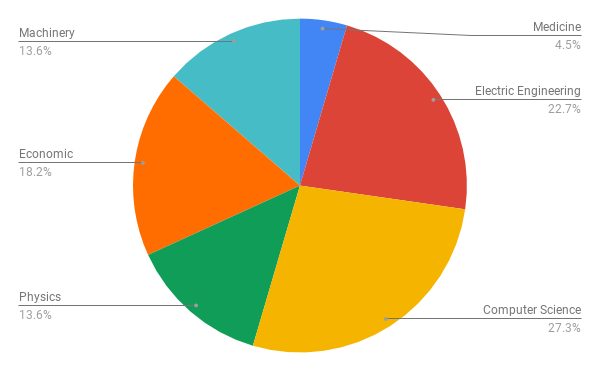
\includegraphics[width=\textwidth]{pictures/q11}
		\caption{Field of study}
	\end{subfigure}
	\hfill
	\begin{subfigure}[b]{0.48\textwidth}
		\centering
		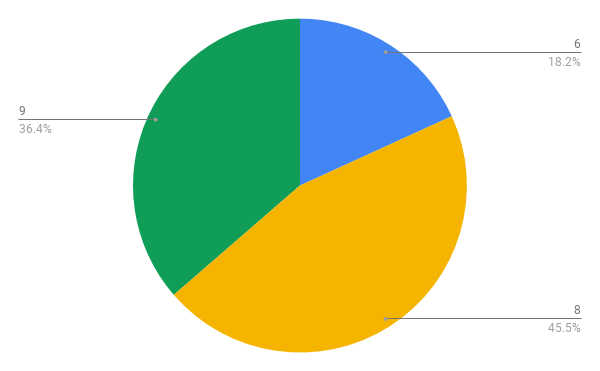
\includegraphics[width=\textwidth]{pictures/q12}
		\caption{Number of semester}
	\end{subfigure}
	\hfill
	\begin{subfigure}[b]{0.48\textwidth}
		\centering
		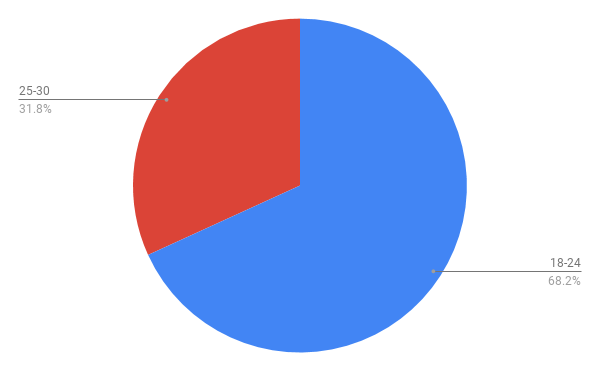
\includegraphics[width=\textwidth]{pictures/q13}
		\caption{Age}
	\end{subfigure}
	\begin{subfigure}[b]{0.48\textwidth}
	\centering
	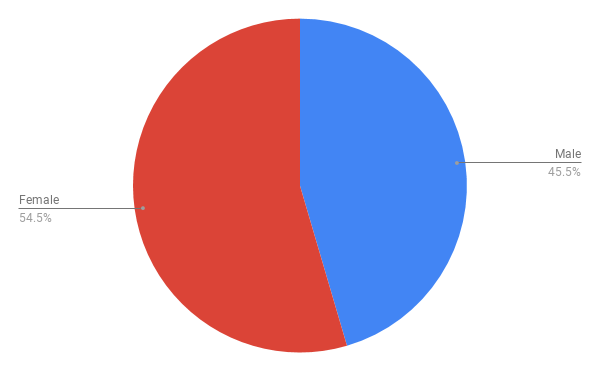
\includegraphics[width=\textwidth]{pictures/q14}
	\caption{Gender}
\end{subfigure}
	\begin{subfigure}[b]{\textwidth}
	\centering
	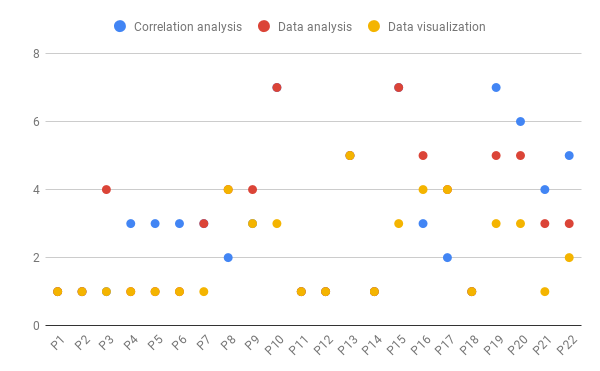
\includegraphics[width=\textwidth]{pictures/q15}
	\caption{How familiar are you with the following concepts?}
\end{subfigure}
	\caption{Statics of basic information}
	\label{fig:statics1}
\end{figure}

\subsection{Statics about the visualization part}
\begin{figure}[h]
	\centering
	\begin{subfigure}[b]{0.48\textwidth}
		\centering
		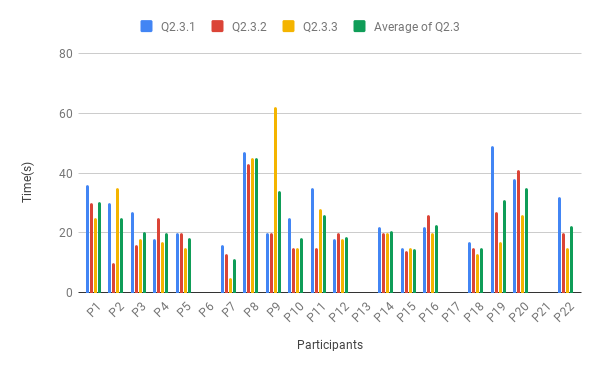
\includegraphics[width=\textwidth]{pictures/q23}
		\caption{Time for Question Q2.3}
	\end{subfigure}
	\hfill
	\begin{subfigure}[b]{0.48\textwidth}
		\centering
		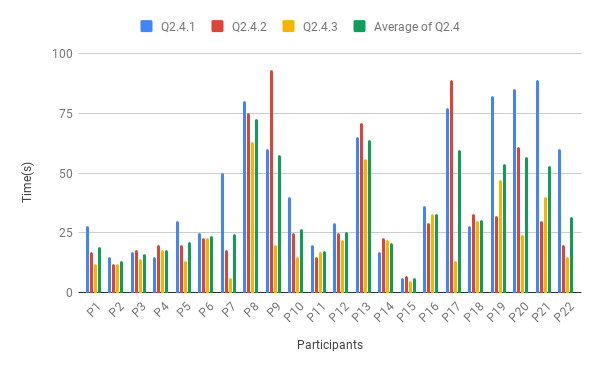
\includegraphics[width=\textwidth]{pictures/q24}
		\caption{Time for Question Q2.4}
	\end{subfigure}
	\hfill
	\begin{subfigure}[b]{0.48\textwidth}
		\centering
		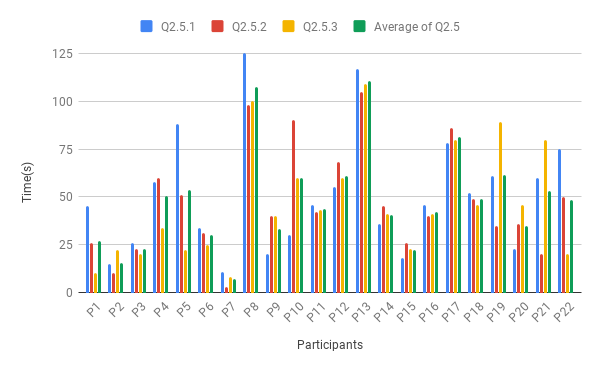
\includegraphics[width=\textwidth]{pictures/q25}
		\caption{Time for Question Q2.5}
	\end{subfigure}
	\begin{subfigure}[b]{0.48\textwidth}
		\centering
		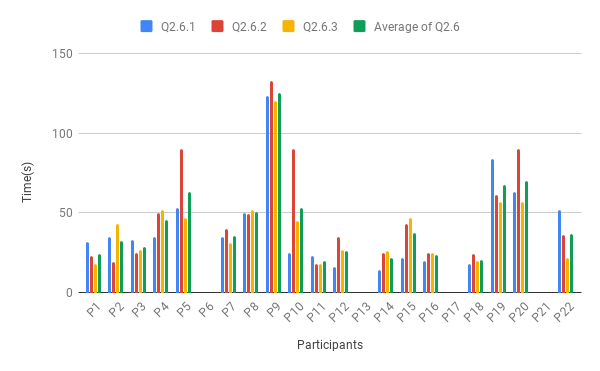
\includegraphics[width=\textwidth]{pictures/q26}
		\caption{Time for Question Q2.6}
	\end{subfigure}
	\begin{subfigure}[b]{0.48\textwidth}
		\centering
		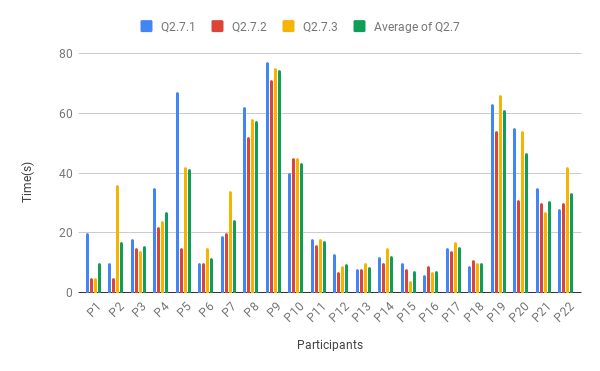
\includegraphics[width=\textwidth]{pictures/q27}
		\caption{Time for Question Q2.7}
	\end{subfigure}
	\begin{subfigure}[b]{0.48\textwidth}
	\centering
	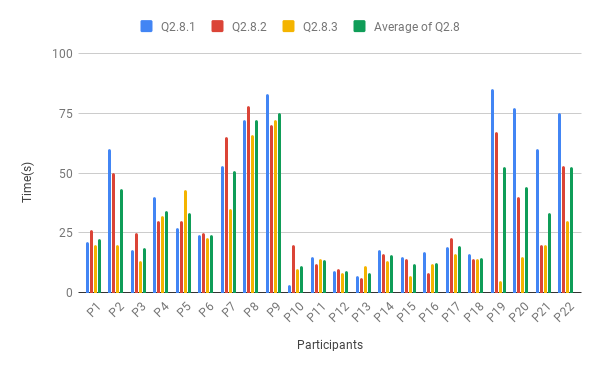
\includegraphics[width=\textwidth]{pictures/q28}
	\caption{Time for Question Q2.8}
\end{subfigure}
	\caption{Time of each participant finishing questions}
	\label{fig:statics2}
\end{figure}

\begin{figure}[h]
	\centering
	\begin{subfigure}[b]{0.48\textwidth}
		\centering
		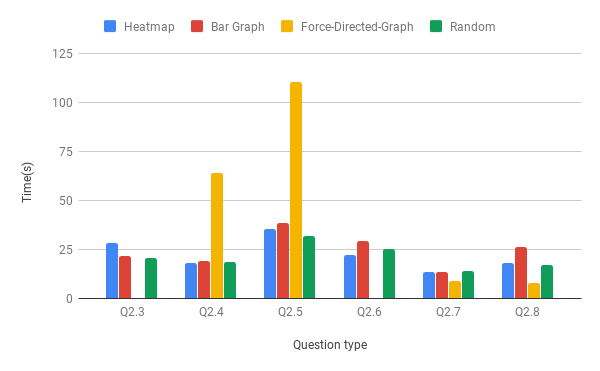
\includegraphics[width=\textwidth]{pictures/Time1}
		\caption{Use Data Set 1}
	\end{subfigure}
	\hfill
	\begin{subfigure}[b]{0.48\textwidth}
		\centering
		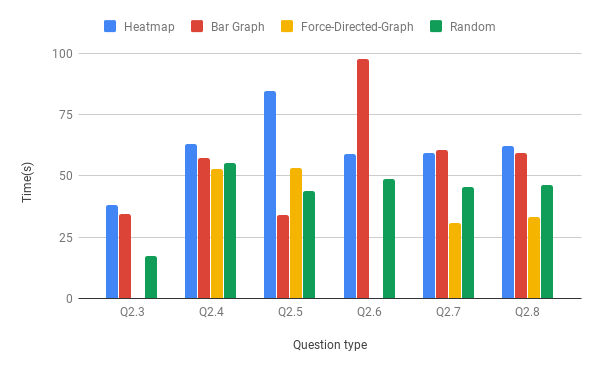
\includegraphics[width=\textwidth]{pictures/Time2}
		\caption{Use Data Set 2}
	\end{subfigure}
	\hfill
	\begin{subfigure}[b]{0.48\textwidth}
		\centering
		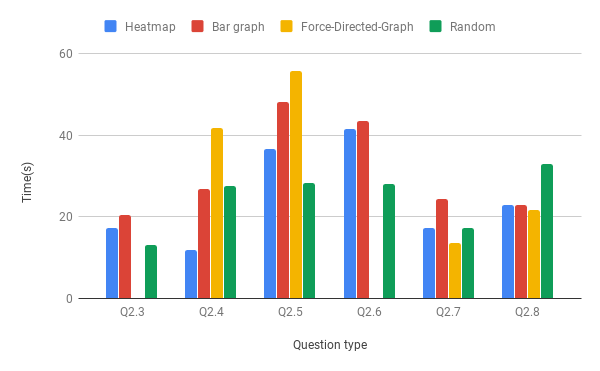
\includegraphics[width=\textwidth]{pictures/Time3}
		\caption{Use Data Set 3}
	\end{subfigure}
	\caption{Average time of participants finishing each question type using different data sets}
	\label{fig:averageDS}
\end{figure}

\begin{figure}[h]
	\centering
	\begin{subfigure}[b]{0.48\textwidth}
		\centering
		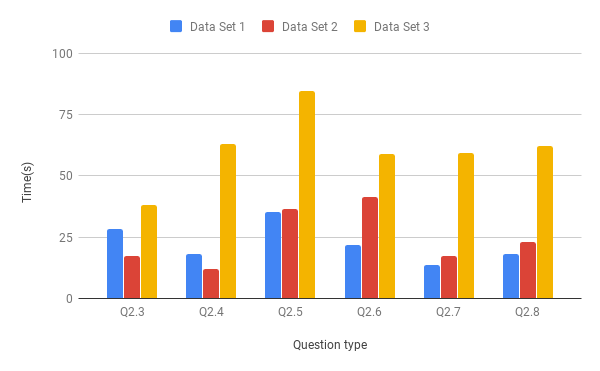
\includegraphics[width=\textwidth]{pictures/TimeH}
		\caption{Use Heatmap as visualization method}
	\end{subfigure}
	\hfill
	\begin{subfigure}[b]{0.48\textwidth}
		\centering
		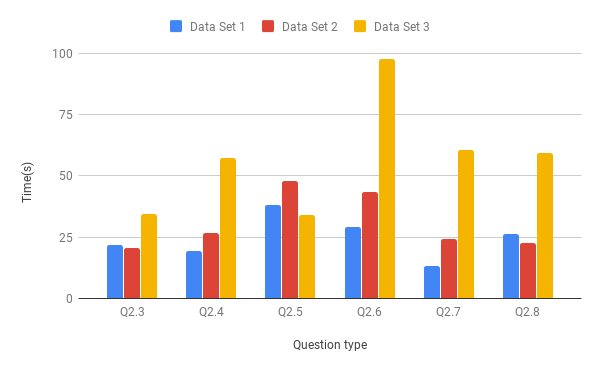
\includegraphics[width=\textwidth]{pictures/TimeB}
		\caption{Use Bar Graph as visualization method}
	\end{subfigure}
	\hfill
	\begin{subfigure}[b]{0.48\textwidth}
		\centering
		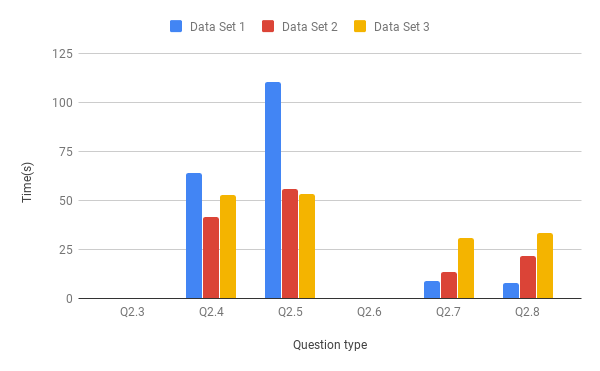
\includegraphics[width=\textwidth]{pictures/TimeF}
		\caption{Use Force-Directed-Graph as visualization method}
	\end{subfigure}
	\begin{subfigure}[b]{0.48\textwidth}
	\centering
	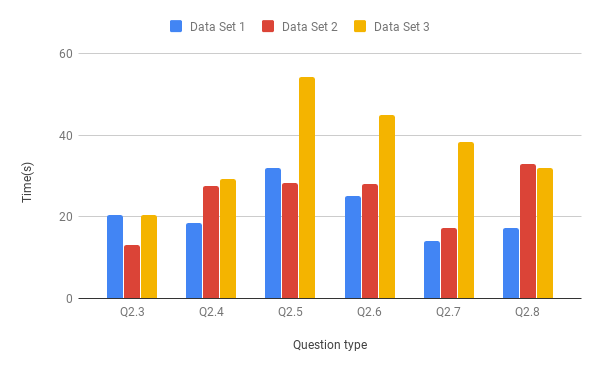
\includegraphics[width=\textwidth]{pictures/TimeD}
	\caption{Use random visualization method}
\end{subfigure}
	\caption{Average time of participants finishing each question type using different visualization methods}
	\label{fig:averageV}
\end{figure}

\begin{figure}[h]
	\centering
	\begin{subfigure}[b]{0.48\textwidth}
		\centering
		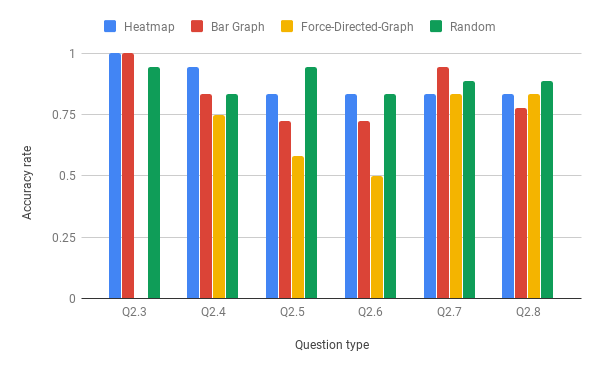
\includegraphics[width=\textwidth]{pictures/accuracy}
		\caption{Accuracy rate of each question type using different visualization methods}
		\label{fig:accuracyV}
	\end{subfigure}
	\hfill
	\begin{subfigure}[b]{0.48\textwidth}
		\centering
		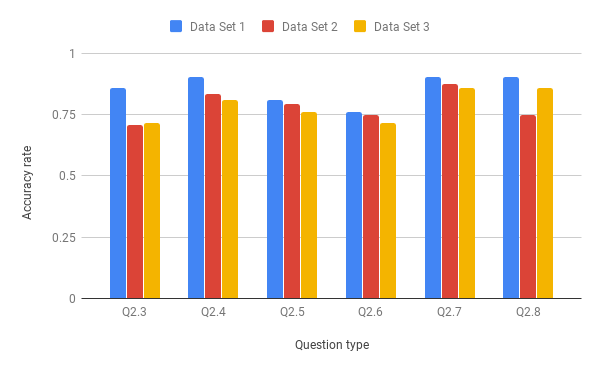
\includegraphics[width=\textwidth]{pictures/accuracyDS}
		\caption{Accuracy rate of each question type using different data sets}
		\label{fig:accuracyDS}
	\end{subfigure}
	\caption{Accuracy rate of each question type}
	\label{fig:accuracy}
\end{figure}

Questions about the number of attributes and pairs of correlations are answered correctly by all the participants. The time they used to answer the other questions are recorded and analyzed in \autoref{fig:statics2}. \autoref{fig:averageDS} shows the statics about the average time of participants using different data sets to finish each question type. It is obvious that both the average time of using Heatmap and Bar Graph is close whatever data set the participants use. When using Force-Directed-Graph, the participants need more time. The time for participants who can use all three visualization methods is also similar to the time using Heatmap/Bar Graph.\\
\autoref{fig:averageV} shows the average time of participants using different visualization methods to finish each question type. We can conclude from the figure that the time for the participants to finish the questions is mostly in direct proportion to the size of the data set, which is also related to the number of pairs for correlations.\\
\autoref{fig:accuracyV} shows the accuracy rate of each question type using different visulization methods. All the accuracy rates are over 50\%. When being able to use Heatmap or 3 visualization methods at random, the accuracy rate even climbs to 75\%. However, for questions asking about the precision, like \textbf{Q2.3}: What is the correlation value between \textit{\textbf{\underline{Attribute A}}} and \textit{\textbf{\underline{Attribute B}}} at \textit{\textbf{\underline{Timestamp T}}}, or the probable range?, the participants are not able to give out their answers by using Force-Directed-Graph. We can infer that Force-Directed-Graph is more suitable to analyze the relationship between attributes than to have a precise value. The accuracy rate of each question type using different data sets is shown in \autoref{fig:accuracyDS}. We can see that using the smallest data set: Data Set 1, always results in the highest accuracy rate.

\subsection{Feedback}
From the survey, we have found out that the Heatmap and Bar Graph are the most often-used visualization methods. We can infer that although they can use three visualization methods in random, they are not quite likely to use Force-Directed-Graph to answer the questions. The ratings for each visualization method and the interface is displayed on the following table:
	\begin{center}
	\begin{tabular}{ | l | l | l | l | l | }
		\hline
		                     & Heatmap & Bar Graph & Force-Directed-Graph & Interface \\ \hline
		\textbf{Intuitive}   & 5.83    & 6.17      & 3.5                  & 6         \\ \hline
		\textbf{Convenient}  & 5.33    & 5.67      & 3.17                 & 5.83      \\ \hline
		\textbf{Interactive} & 5.83    & 5.67      & 4.17                 & 6.16      \\ \hline
		\textbf{Useful}      & 6       & 5.67      & 3.33                 & 5.83      \\ \hline
		\textbf{Complicated} & 2.67    & 3         & 4                    & 3.17      \\ \hline
		\textbf{Efficient}   & 5.33    & 5         & 3.33                 & 5.83      \\ \hline
		\textbf{Effective}   & 5.5     & 5.67      & 3.67                 & 5.67      \\ \hline
	\end{tabular}
\end{center}
From the table, we can see that the Force-Directed-Graph is the most complicated visualization methods for participants. Most participants found Heatmap and Bar Graph very intuitive in data visualization. In the feedback, intuition is one of the strength of this visualization system. In addition, this system meets many demands for data processing. As we have three visualization methods, each method can be used for different use to ease the correlation analysis. It is also interesting to see the change of graphs by sliding the sliding window.\\
The maximal value is very easy to find out by the interface, but when it comes to a relative small correlation value, it is quite hard for participants. Although different color of blocks represents different value in Heatmap, the blocks looks the same when the difference of two values is small, e.g. 0.005. Also, when the number of correlations is big, it's labored to see through the bars to find the change of one pair of attributes. Thanks to the filtering of minimal and maximal values of correlation values, the participants can save some time and strength to analyze the data.\\
The participants are glad to see more visualization methods and to use more functions of this interface. It is suggested that the interface is not only used for correlation analysis, but also for data analysis and have functions like mean, variance and median. Also, it could be helpful to output the exact correlation value of one pair by inputting the names of attributes. For Bar Graph, sort functions to re-arrange the order is quite useful to find certain pairs. As the Force-Directed-Graph shows the relationships of attributes, it is interesting when one node is pointed, only the related links will be shown. Also, only showing small sub-groups of the attributes can be helpful.